\documentclass{article}
\usepackage[utf8]{inputenc}
\usepackage{amsmath,amssymb}
\usepackage{amsfonts}
\usepackage{paralist}
\usepackage{color}
\usepackage[table]{xcolor}
\usepackage{graphicx}
\usepackage{pgfplots}
\usepackage{authblk}
\usepackage{url}
\usepackage{multirow}
\usepackage{booktabs}
\usepackage{blindtext}
\usepackage{adjustbox}
\usepackage{subcaption}
\usepackage[margin=1.3in]{geometry}

\usepackage{float}
\usepackage[font=small, labelfont=bf, textfont=it, format=hang]{caption}
\usepackage[colorlinks=true, allcolors=blue]{hyperref}
\urlstyle{same}
\usepackage[english,nameinlink]{cleveref}
\usepackage{natbib} 
\crefname{equation}{}{}

\title{HPC Final Project}
\author{Valentinis Alessio [SM3800008]}
\date{27/02/2024}

\begin{document}
	\maketitle
	\tableofcontents
	
	\part{Exercise 1}
	
	The goal of the exercise is to estimate the latency of default openMPI implementation of two collective blocking algorithms, one of which being \textit{broadcast}, varying the virtual topology with which the algorithms operate, along with the map by whcich the cores are allocated.
	My choice resided into:
	\begin{itemize}
		\item \textbf{Broadcast}: varying virtual topologies among \textit{default}, \textit{basic linear}, \textit{flat chain} and \textit{binary tree}.\\
		\item \textbf{Barrier}: varying virtual topologies among \textit{default}, \textit{basic linear}, \textit{double ring} and \textit{bruck}.
	\end{itemize}
	
	The benchmark library used is OSU microbenchmark, available \href{https://mvapich.cse.ohio-state.edu/benchmarks/}{here}.
	The tests were conducted on the EPYC nodes in the ORFEO clusters and all tests were performed following a \textit{bash} script to automatize the process of data gathering.
	
	\section{Broadcast operation}
	
	MPI\_Broadcast is a fundamental collective communication operation provided by the Message Passing Interface (MPI) library. It allows one process, typically referred to as the root process, to efficiently broadcast data to all other processes in a communicator. This operation is crucial for distributing information across multiple processes in parallel computing environments. It's a widely used one-to-all operation that, by default is implemented in multiple ways, in order to optimize the process of sending data to multiple processes.
	We will go into some further details only of those operations which are covered in this study.
	\begin{itemize}
		\item Default: this kind of implementation should authomatically choose the optimal way of sending the information, based on both size of the message and number of cores.\\
		\item Basic linear: it's the way we could think to implement the broadcast algorithm, i.e. the root process sends sequentially to all processes the message, one by one.\\
		\item Chain: In this implementation, as the name suggests, the message is sent from one process to the other, so process0 sends its message to process1, process1 to process2, and so on and so forth.\\
		\item Binary tree: as the name suggests, this virtual topology of the cores is such that they are places in a binary tree fashion, so process0 is in charge of sending the message to process1 and process2, process1 to process3 and process4, and so on.
	\end{itemize}
	
	For some of these operations message segmentation is inabled, so the message is divided in chunks, and these chunks are sequentially sent to the other processes. In particular we are referring to binary tree and chain.
	
	\subsection{Data collecting process}
	The process of collecting data has been authomatized through the use of a bash script, available in the GitHub \href{https://github.com/ValentinisAlessio/HPC_final_project}{repository}. 
	To have a better view of the what happens with different mappings of the cores, the same gathering process has been brougth on varying the \textit{--map-by} parameter, and to collect as many data in one shot, the maximum message has been truncated to 2024 bytes, which is anyway well beyond the latency-dominated size region.
	To allow for a better data gathering process, the different mapping of the cores (by core, by socket and by node), the different scripts have been separated.
	
	As previously announced, the tests have been brought up into the EPYC nodes, selecting and prioritizing the acces to two whole nodes. So, due to the characteristics of the computing architecture, I have conduced the test onto a maximum of 256 cores, distributed in four sockets and two nodes.
	
	To have better quality of the data collected, I chose to set 100 warmup operation and 10000 effective operations, from which the average has been taken and recorded.
	
	\subsection{Latency analysis}
	
	The data collection process generated a pretty substantial dataset, providing different combinations for algorithm, cores allocation and message size to analyze the average latency of the communication.
	To tackle this complexity and various combinations, my effort was to sequentially fix some degrees of freedom, while varying the others, one or more at the time. At the end I tried to develop a model that could explain the interaction between the various covariates and the Average Latency measurements.
	
	\subsubsection{Fix algorithm and vary allocation}
	
	In this part we explore the behavior of the various algorithm, for data size of 1 MPI\_CHAR, so 1 byte, by varying the number of cores and cores allocation. This choose of the message size isolates and examines the "pure" latency of the communication.
	
	% INSERIRE IMMAGINE DI ALGORITMI PER 1 CHAR communications
	% 1a default
	% 1b linear
	% 1c chain
	% 1d binary
	
	\begin{figure}[h]
		\centering
		\begin{subfigure}{0.45\textwidth}
		\centering
		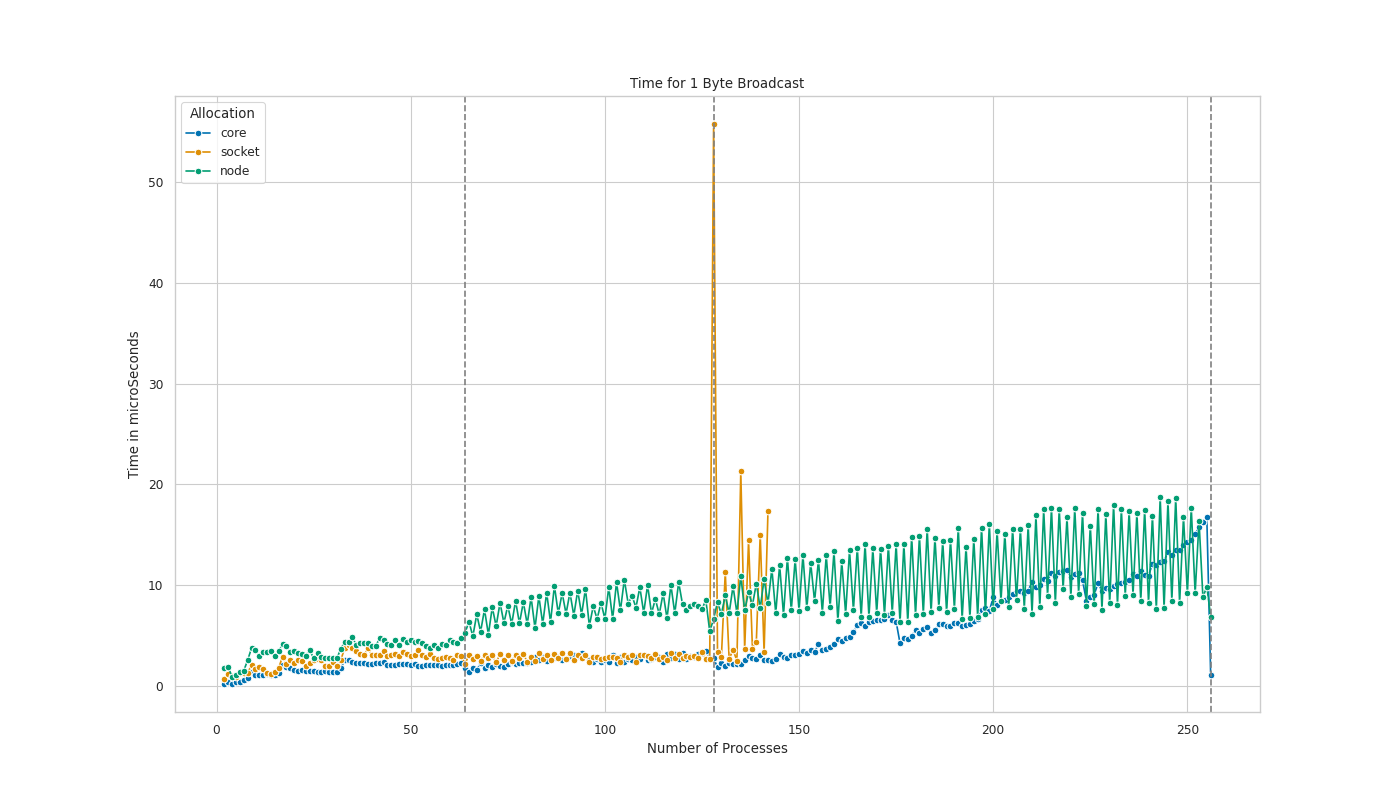
\includegraphics[width=0.7\linewidth]{../exercise1/plots/bcast_default_1byte}
		\caption{Average Latency vs n. processes in default algorithm}
		\label{fig:bcastdefault1byte}
		\end{subfigure}
		\begin{subfigure}{0.45\textwidth}
			\centering
			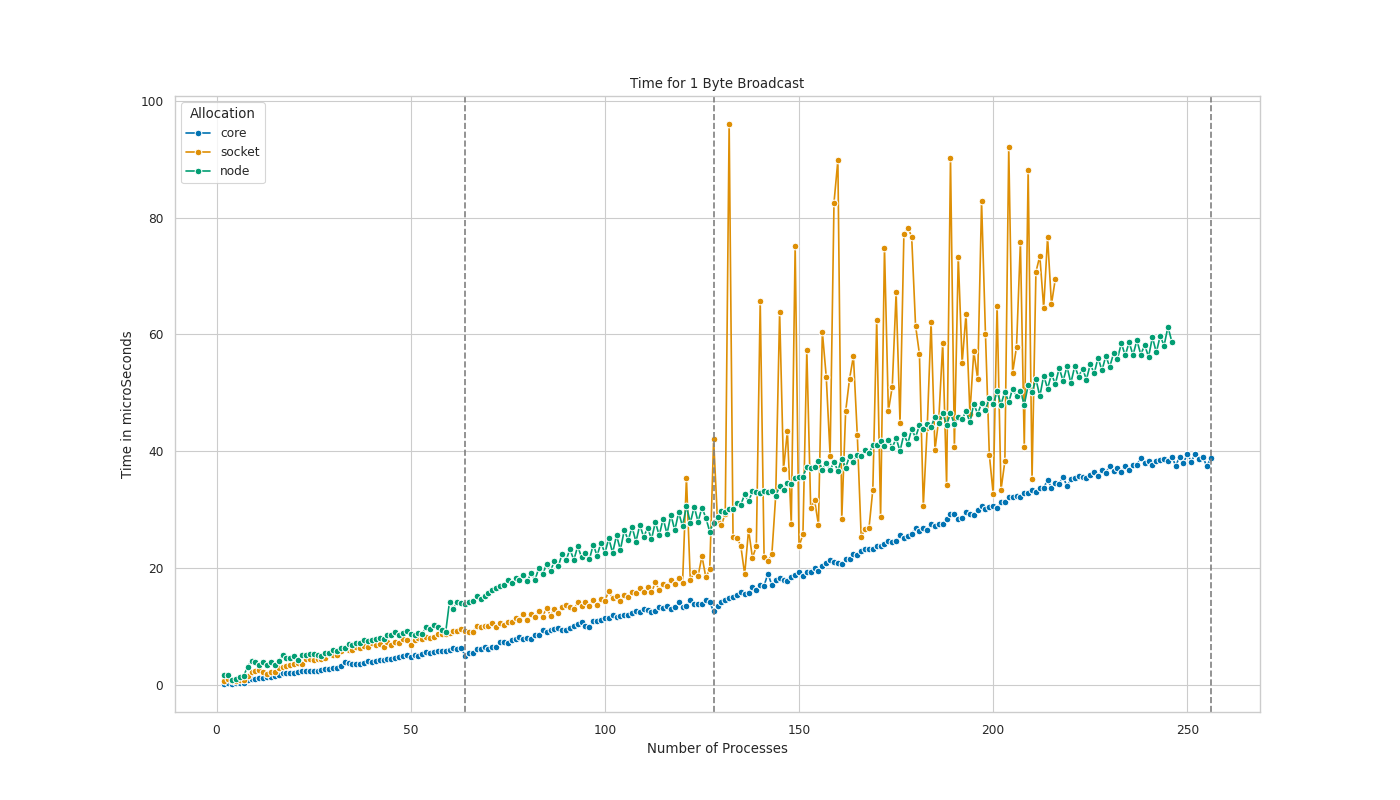
\includegraphics[width=0.7\linewidth]{../exercise1/plots/bcast_linear_1byte}
			\caption{Average Latency vs n. processes in linear algorithm}
			\label{fig:bcastlinear1byte}
		\end{subfigure}
		\begin{subfigure}{0.45\textwidth}
			\centering
			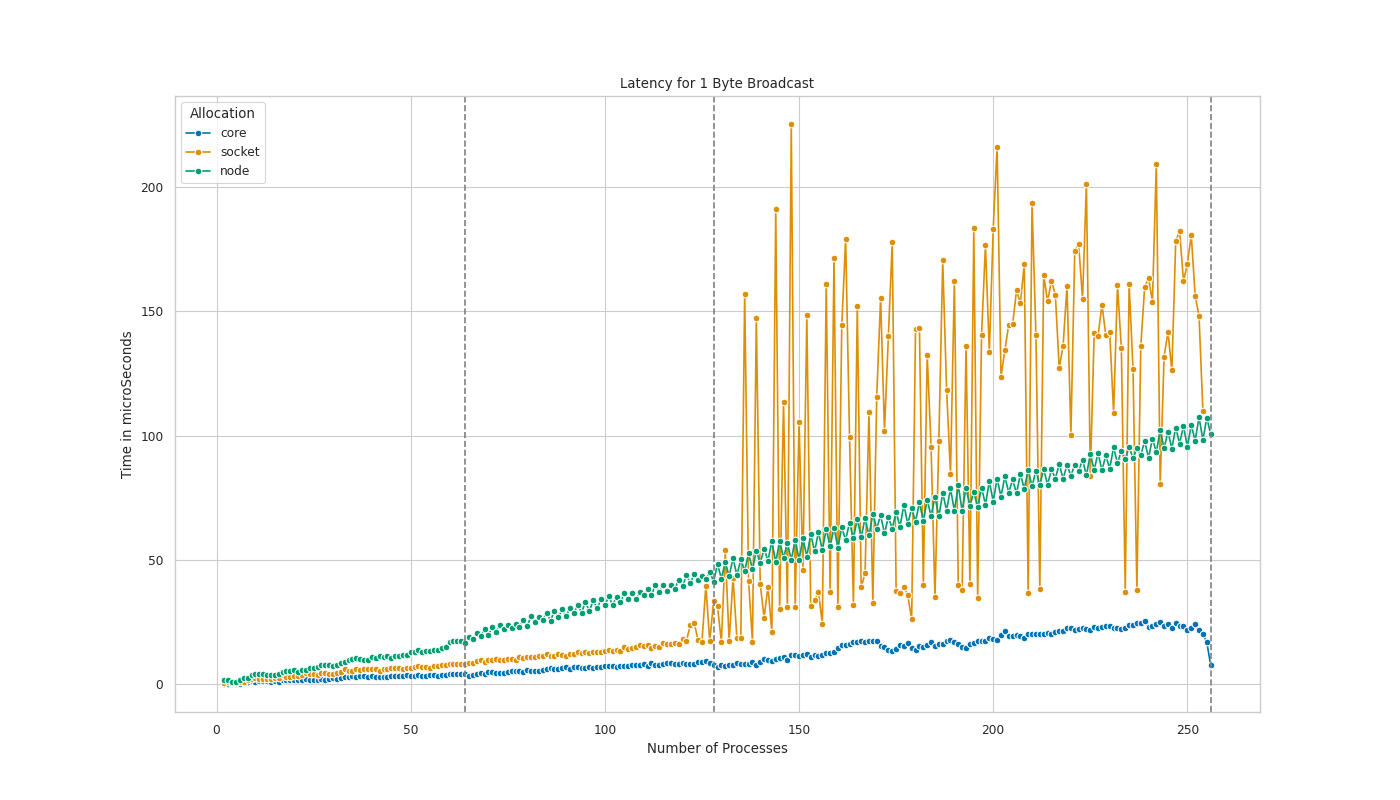
\includegraphics[width=0.7\linewidth]{../exercise1/plots/bcast_chain_1byte}
			\caption{Average Latency vs n. processes in chain algorithm}
			\label{fig:bcastchain1byte}
		\end{subfigure}
		\begin{subfigure}{0.45\textwidth}
			\centering
			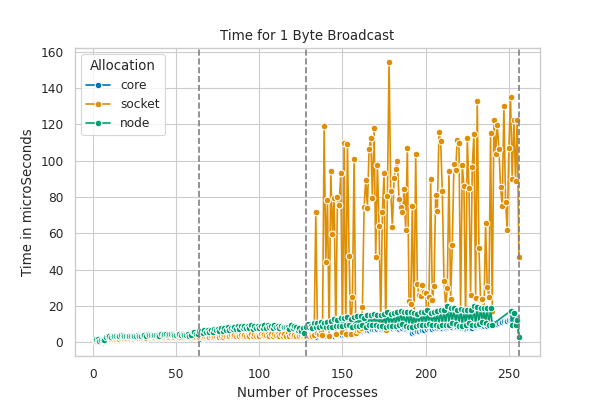
\includegraphics[width=0.7\linewidth]{../exercise1/plots/bcast_bintree_1byte}
			\caption{Average Latency vs n. processes in binary tree algorithm}
			\label{fig:bcastbintree1byte}
		\end{subfigure}
	\end{figure}
	
	
	
	Concerning the first plot, default algorithm behaves as expected, as we can clearly identify three regions, above all in core and socket mappings, with two noticable jumps and changing in behavior, while node allocation doesn't show remarkable and noticable jumps. The two jumps happen almost where expected, so at 64 cores, when we change socket, and at 128 cores, when we completely change node. It's worth to notice that the jump at the change of socket is by far more accentuated in the core mapping, as in that scenario cores are allocated as close as possible in the same socket. 
	
	Passing at the second plot, regarding the basic linear algorithm, we can observe almost the same behaviour at least for the core and node mapping. In socket mapping we can see that the change of behavior doesn't happen exactly at 128 cores as expexted, suggesting some more complicated model beyond "naive" node/socket changes.
	
	Going to the chain algorithm some similar observations to the previous ones hold, but with some peculiarities.
	In fact, differently from the previous ones, we can see the "serial" nature of the comunication, as the different positioning of the processes deeply impact on the latency measurements, with the node allocation by far diverging from the other two, at least in the one-node situation.
	
	Lastly, going to the binary tree algorithm, the lower latency measurements underscore and emphasize its (expected) superiority compared to the other algorithms. Moreover, we can see that allocating processes by node, we obtain some more stable latency when surpassing the 128 cores, showing some kind of optimized communication when dealing with processes inside the same node.
	Allocating by core or socket, instead, shows some jumps followed by immediate decreases in latency corresponding to the "region change" thresholds, which explanation may reside inside the hierarchical nature of the algorithm. In fact these phenomena could be due to the transition between two different levels of the tree, that may introduce some delay in the communication. Once this transition is passed, the latency decreases, as the subsequent level of the tree gets filled.
	
	\subsubsection{Compare algorithms fixing allocation}
	
	In this second part of our analysis, we fixed the allocation type to \textit{core}, as it shows all the expected changes in behavior of the algorithm, and is the less influenced by eventual iner-node traffic with other communication. Fixing this degree of freedom, we chose once more to analyze the 1 byte scenario, to isolate the pure latency of the communication, and we vary number of cores and type of algorithm.
	
	% INSERT IMAGE OF ALL MAP BY CORE
	\begin{figure}[h]
		\centering
		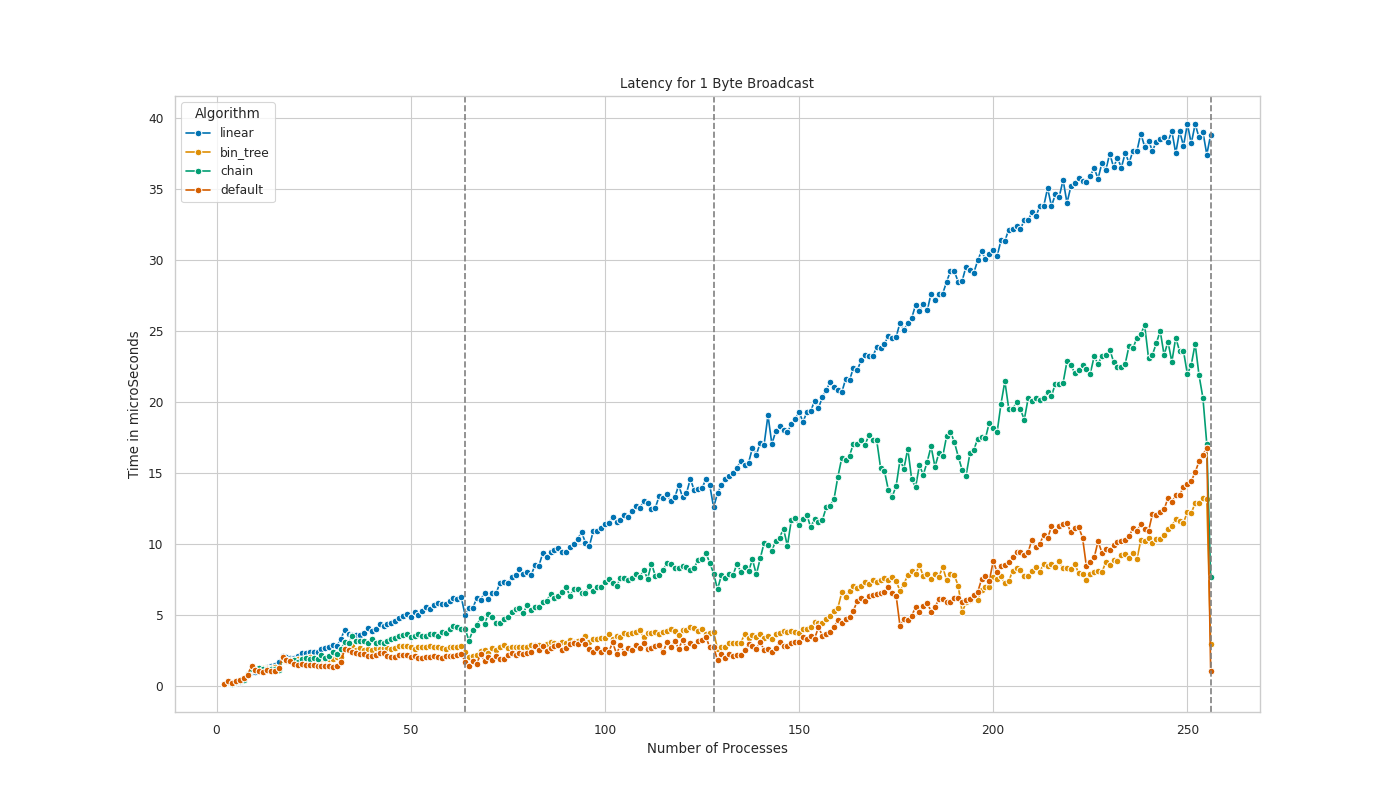
\includegraphics[width=0.9\linewidth]{../exercise1/plots/bcast_all_1byte}
		\caption{Latency vs n. processes by algorithm}
		\label{fig:bcastall1byte}
	\end{figure}
	
	
	The figure above offer some insights into how the algorithm influences across three main regions:
	
	\begin{itemize}
		\item \textbf{Within 64 cores}: in this intra-socket region we can observe almost identical performances, which can be indicative of some optimal speed of communication occuring between cores in the same socket. The slight advantage observed with respect to the default and binary tree algorithm may be due to the fact that the first selects the send policy authomatically, while the latter organizes in a more optimal way the hierarchy of communication.\\
		\item \textbf{From 64 to 128 cores}: in this intra-node region we can begin to observe some more consistent advantage in terms of latency of the two algorithm mentioned above, which suggests that in this situation a choice among implementation may be done.
		\item \textbf{Above 128 core}: in this region we enter inter-node communication, and we can clearly state that the performance of the linear algorithm gets worse and worse, suggesting that with more processes to manage, the binary tree algorithm gains more than something in terms of performance, as the communication is done by a hierarchy processes, and not by one to all.
	\end{itemize}

	\subsubsection{Fixing allocation and vary message size}
	
	In this section we plan to analyze the various performance models among different message size.
	
	% INSERT IMAGES ABOUT DIFFERENT MESSAGE SIZES
	\begin{figure}[h]
		\centering
		\begin{subfigure}{0.45\textwidth}
			\centering
			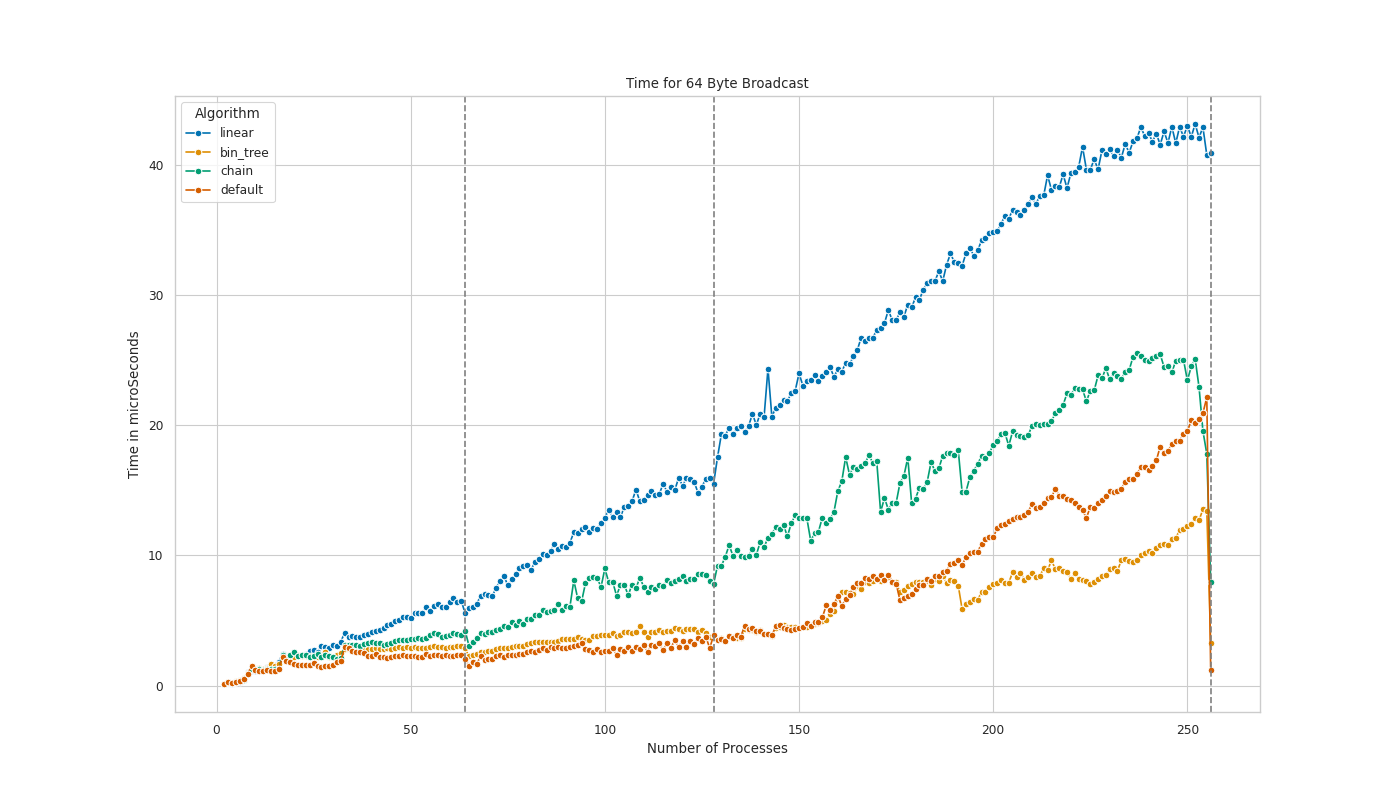
\includegraphics[width=0.7\linewidth]{../exercise1/plots/bcast_all_64byte}
			\caption{Average Latency vs n. processes for 64 byte message}
			\label{fig:bcastall64byte}
		\end{subfigure}
		\begin{subfigure}{0.45\textwidth}
			\centering
			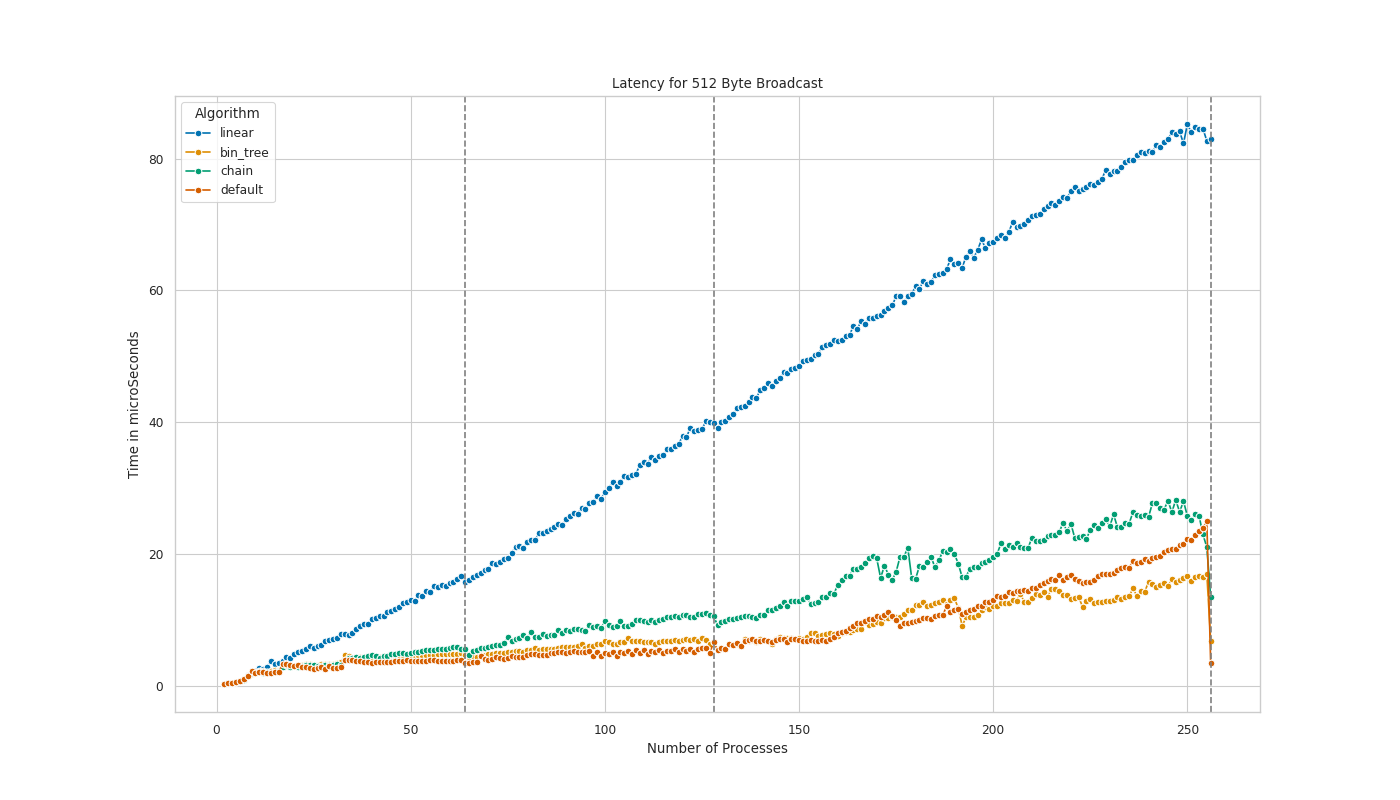
\includegraphics[width=0.7\linewidth]{../exercise1/plots/bcast_all_512byte}
			\caption{Average Latency vs n. processes in 512 byte message}
			\label{fig:bcastall512byte}
		\end{subfigure}
		\begin{subfigure}{0.45\textwidth}
			\centering
			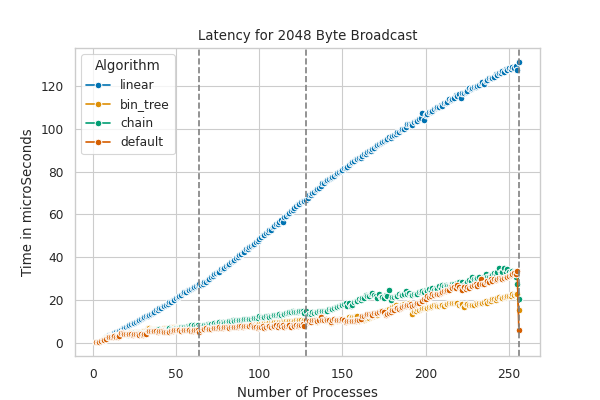
\includegraphics[width=0.7\linewidth]{../exercise1/plots/bcast_all_2048byte}
			\caption{Average Latency vs n. processes in 2024 byte message}
			\label{fig:bcastall2048byte}
		\end{subfigure}
	\end{figure}
	
	Varying message sizes we can observe more peculiar aspects of each implementations: while with a 1 byte message, the difference between implementations is pretty negligible as long we remain into the same node, varying message sizes, we can clearly see how the linear algorithm performs wprse and worse increasing the message size.
	This behavior is due to two main factors: firstly the communication between processes is put as responsibility of the root process, which one by one sends the message to the other processes, while in all other algorithms the communication is organized in a more or less hierarchical way; secondly the linear approach is the only one among the analyzed ones that doesn't imply message segmentation, so in the linear algorithm the message is sent entirely from the root process to the remaining ones. The other methods, on the other hand, aside from the hierarchy of communications, allow for message segmentation, i.e. the message is divided in chunks and sent one chunk at the time via buffer-send (MPI\_ISend), as mentioned in the article (\textit{Here put link to article in the github repo of HPC}).
	
	\subsection{Broadcast performance model}
	As a conclusive step of the analysis I attempted to formulate a performance model to try to better understand the not-so-straight-forward dynamics playing into these algorithms. 
	At firt I gave a try at estimating both latency and bandwidth within point-to-point communications employing again the OSU-microbenchmark library. The intention was to try and develop the Hockney model I found explained in some articles. However, the results obtained didn't fit well with the collected data, suggesting me to try something different. Maybe biased by my mathematical backgroud, or by some freshly sustained exams, I opted for the implementation of a linear model.
	
	% INSERISCI PARTE RIGUARDO MODELLO LINEARE
	
	
	\section{Barrier operation}
	
	In this second part of the exercise, I chose to analyze and study the performance model of the MPI\_Barrier algorithm. It's an operation that allows for the synchronization of different process within the same communicator. It consists in a construct that guarantees that by the end of the operation, all the processes have at least entered the operation.
	This collective blocking operation becomes crucial when we want to synchronize the processes involved in some parts of our distributed programm to ensure coherent and predictable execution. Among the plethora of synchronization mechanisms, the barrier algorithm stands as a fundamental construct, enabling synchronization points within parallel programs.
	By default, the library OpenMPI offers different implementation of this algorithm, always characterized by beculiar virtual topology of the cores, or by different hierarchy of the execution. In this study I have examined only four of the  several algorithms present.
	
	\begin{itemize}
		\item Default: this kind of implementation chooses authomatically the optimal way to synchronize the processes, based on their number and allocation.\\
		\item Linear: in this algorithm all nodes refer to a preselected root; once everyone has reported to the root, it sends a release message to everyone.\\
		\item Double Ring: in this algorithm, a zero-byte message is sent from a preselected root to its right circularly; a node can leave Barrier once it receives the message for the second time.\\
		\item Bruck algorithm: this implementation, alternatively from the two just descripted, which require $P$ communication steps, only requires $\lceil log_2P \rceil$. At a generic step $k$, process $r$ receives zero-byte message from and sends the same message to process $r - 2^k$ and $r + 2^k$ respectively. This process goes on untill each process have received the message from all other processes.
	\end{itemize}
	
	\subsection{Data collecting process}
	
	The process of collecting data, similarly to the first part, has been authomatized through the use of a bash script. To ensure a better all around view of the process, the same gathering process has been brought up on varying the \textit{--map-by} parameter. To allow the generation of a more complete dataset, the different scripts are divided other than by algorithm, also by core mapping.
	
	As before, the tests have been conducted into the EPYC nodes, selecting two whole computing nodes fully reserved for this task.
	
	Similarly of what happened in the first part, to have more consistent and less biased data, I chose to select 100 warm up operations and 10000 effective misurations, from which the average has been taken and recorded.
	
	\subsection{Latency analysis}
	
	The data collection process generated a complete dataset, that can in principle allow for a quite extensive analysis. Similarly to the first part, my effort was to select and fix some degrees of freedom , while varying the others, and permitting for a simpler visualization of the data.
	At the end I tried to formulate a model that could explain the complex interaction between the various parameters.
	
	\subsubsection{Vary allocation for fixed algorithm}
	
	In this part we are going to explore the behavoiur of the various algorithms, by varying number of processes and core allocation.
	
	% INSERIRE IMMAGINE DI ALGORITMI PER 1 CHAR communications
	% 1a default
	% 1b linear
	% 1c ring
	% 1d bruck
	
	\begin{figure}[h]
		\centering
		\begin{subfigure}{0.45\textwidth}
			\centering
			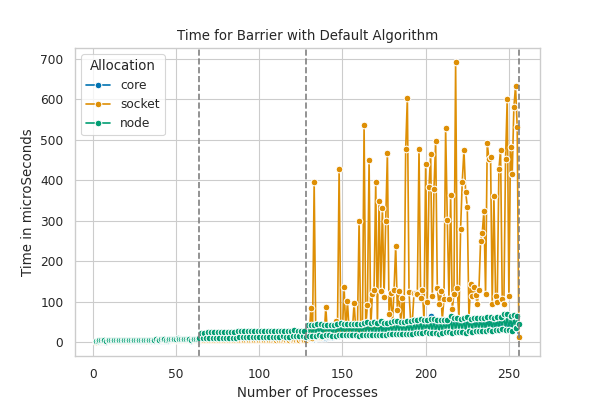
\includegraphics[width=0.7\linewidth]{../exercise1/plots/barrier_default}
			\caption{Average Latency vs n. processes in default algorithm}
			\label{fig:barrierdefault}
		\end{subfigure}
		\begin{subfigure}{0.45\textwidth}
			\centering
			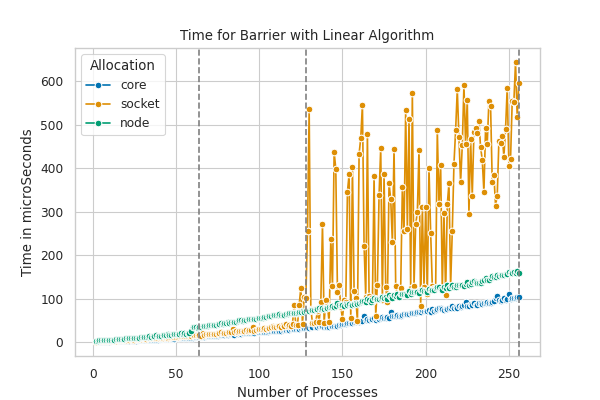
\includegraphics[width=0.7\linewidth]{../exercise1/plots/barrier_linear}
			\caption{Average Latency vs n. processes in linear algorithm}
			\label{fig:barrierlinear}
		\end{subfigure}
		\begin{subfigure}{0.45\textwidth}
			\centering
			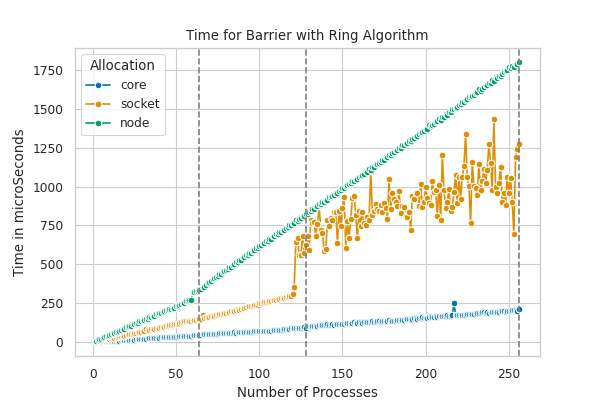
\includegraphics[width=0.7\linewidth]{../exercise1/plots/barrier_ring}
			\caption{Average Latency vs n. processes in double ring algorithm}
			\label{fig:barrierring}
		\end{subfigure}
		\begin{subfigure}{0.45\textwidth}
			\centering
			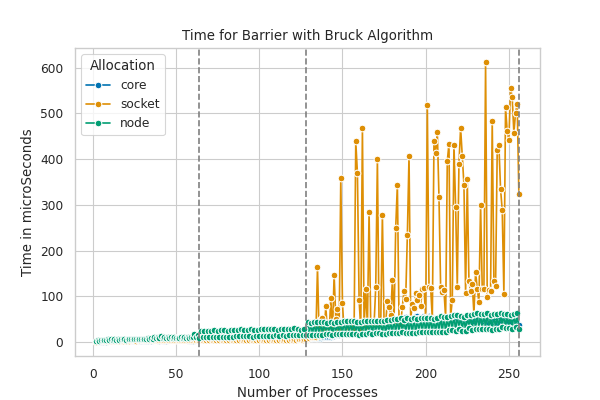
\includegraphics[width=0.7\linewidth]{../exercise1/plots/barrier_bruck}
			\caption{Average Latency vs n. processes in bruck algorithm}
			\label{fig:barrierbruck}
		\end{subfigure}
	\end{figure}
	
	Concerning the first plot we can clearly identify three different regions, one with less than 64 cores, where the three allocations seem to encounter the same latency, a secon up to 128 cores, where node allocations shows some worse behavior, and a third, when we exceed the number of processes into one node, where the socket allocation goes crazy while node distribution gains something with respect to core one. It's worth notice that, contrary to the broadcast algorithm, we cannot notice remarkable jumps in latency when we pass through some thresholds, as we are dealing with a zero-sized message communication among all processes.
	
	Passing to the second plot, regarding the linear algorithm, we can see almost the same characteristics as before, just with some more regular pattern into the node allocation. We can see that the changes in behavior don't happen where expected, suggesting some more complex interaction than the simple node/socket changes.
	
	Going to the Double Ring algorithm, we can see some pretty worse behavior in general, with hugher values of the latency, and with clear separation between the three types of allocations. This may be due to the "serial" nature of the communication, where process0 waits for process1, which waits for process2, and so on and so forth untill each process receives the message for the second time. This reflects in an almost linear behavior in all the types of allocation, with the node distribution being from the beginning the worst one.
	
	Lastly, passing to the bruck algorithm, we can see some similar behavior to the default algorithm, with the same region division and almost the same behavior, suggesting that this algorithm may have an optimal hierarchy of communication, making it suitable for the default implementation.
	
	\newpage
	
	\subsubsection{Compare algorithms fixing allocation}
	
	In this second part of our analysis, we fixed the core allocation to \textit{core}, which showed to be more stable, other than being the least influenced by inter-node traffic.
	
	% INSERIRE IMMAGINE DI TUTTI GLI ALGORITMI MAPPATI PER CORE
	
	\begin{figure}[h]
		\centering
		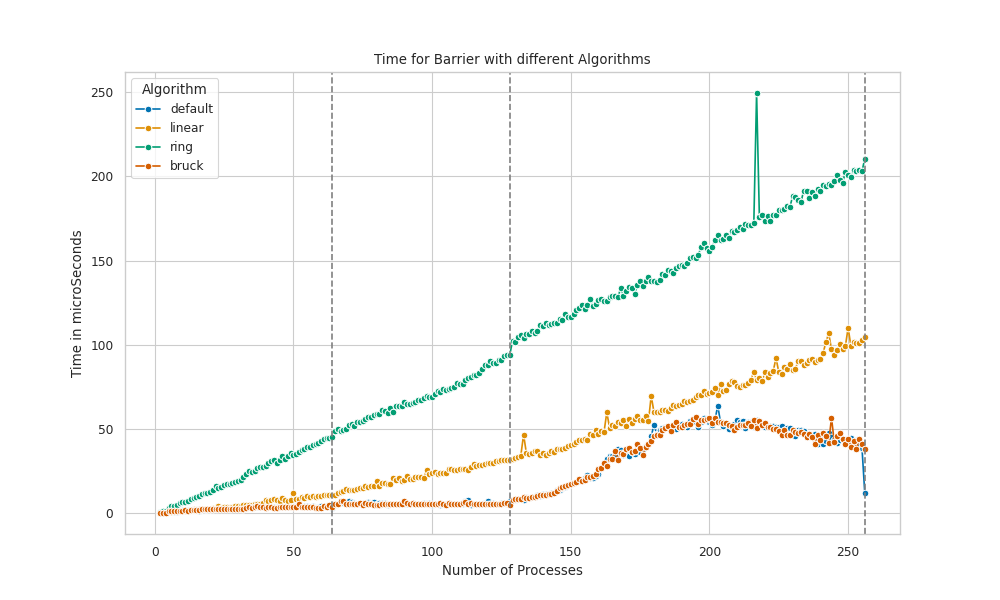
\includegraphics[width=0.9\linewidth]{../exercise1/plots/barrier_core}
		\caption{Latency vs n. processes by algorithm}
		\label{fig:barriercore}
	\end{figure}
	
	The figure above illustrates the four algorithms analyzed and offers some points of analysis straight away:
	
	\begin{itemize}
		\item Linear behaviors: we can clearly see as the double ring and linear algorithms have a quite consistent linear trend, justifying the linear number of communication required to complete the operation.
		\item Logarithmic trends: we can also see as the default and bruck implementation behave almost in the same way, suggesting that the latter is preferred. To justify the trend of the latency measurements, we have to take into consideration the bruck algorithm, where each process has to manage $log_2P$ Send operations. So within the same node we can see almost clearly the logarithmic behavior of the latency, while whe trepassing the node limit, due also to the inter-node latency in the communication, we have a "jump", and the same logarithmic trend reestablish when we have enough cores into the second node.
	\end{itemize}
	
	\subsection{Barrier performance model}
	
	Similar to the first part of the exercise, in this section my aim is to develop a statistical model that can explain the latency measurements as a function of the others degrees of freedom.
	
	% INSERIRE PARTE DI ANALISI STATISTICA
	 
\end{document}